Vamos a analizar el caso de las consultas en rango para un segment tree de suma. Recibimos dos enteros $a$ y $b$ que representan los l\'imites del rango al que hay que calcularle la suma en un tiempo proporcional a $O(\log n)$.

\begin{corollary}[Consulta en Rangos]

    Nuestro pro\-ce\-di\-mien\-to es recursivo. Comenzamos en el v\'ertice ra\'iz. Cuando llegamos a un nodo $v$ cuyo rango es $[l, r]$, tenemos tres casos posibles:

    \begin{enumerate}
        \item{
            \textit{Si el intervalo $[l, r]$ del nodo est\'a completamente DENTRO del intervalo $[a, b]$:} Se retorna el resultado co\-rres\-pon\-dien\-te al v\'ertice actual (en este caso la suma), ya que este resultado debe ser tomado en cuanta para calcular la respuesta final.
        }
        \item{
           \textit{Si el intervalo $[l, r]$ del nodo est\'a completamente FUERA del intervalo $[a, b]$:} Se retorna un valor que no modifique la respuesta final. Como estamos calculando la suma, este valor es el cero.
        }
        \item{
            \textit{Si no se cumple NINGUNA de las condiciones anteriores:} Entonces llevamos a cabo este procedimiento en los hijos del nodo actual y luego combinamos la respuesta de cada ve\'rtice hijo, de ah\'i la naturaleza recursiva de este algoritmo.
        }
    \end{enumerate}

\end{corollary}



Para el ejemplo del arreglo $\{2, 3, 1, 6, 2, 1\}$, y la consulta de la suma del rango $[1, 5]$, comenzar\'iamos en el nodo del intervalo $[1, 6]$. Este nodo no cumple ninguna de los dos primeros casos, por lo que aplicando el tercero, llamamos a la funci\'on recursivamente en sus hijos.

\begin{minipage}{\columnwidth}
    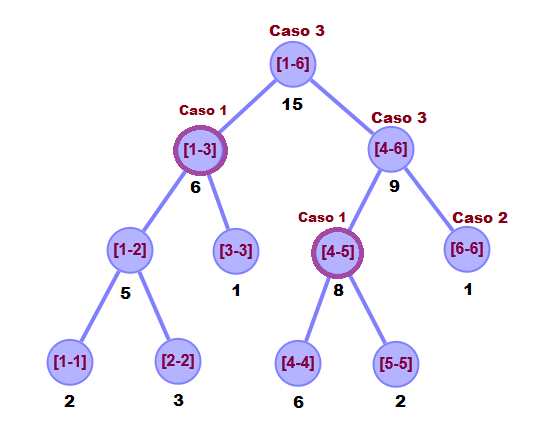
\includegraphics[width=\linewidth]{imag/segment_tree_query_casos}
    \label{fig:example_st_casos}
\end{minipage}

Para el hijo izquierdo, correspondiente al intervalo $[1, 3]$ se cumple la primera regla, porque el intervalo del nodo est\'a completamente dentro del intervalo de la consulta. Entonces retornamos el resultado precalculado de este v\'ertice. En este caso no hacemos m\'as llamadas recursivas en los hijos de este nodo.

El hijo derecho de la ra\'iz solo cumple la regla $3$, por lo que aplicamos el procedimiento a sus hijos. Para el nodo correspondiente al intervalo $[4, 5]$ se cumple la regla $1$. Entonces retornamos su valor precalculado. Para el nodo del rango $[6, 6]$ se cumple la regla $2$, por lo que devolvemos un valor que no modifique la respuesta; en este caso ese valor es el cero. 


Vamos a repasar los valores que obtuvimos en cada nodo: En el nodo del intervalo $[1, 3]$ obtuvimos el valor $6$. En el nodo del intervalo $[4, 5]$ obtuvimos el valor $8$ y en el nodo del intervalo $[6, 6]$, el valor cero. La suma de estos valores es la respuesta a la consulta: $6 + 8 + 0 = 14$.

Hay que aclarar que \textbf{los valores que se calculan para cada nodo en las consultas en rangos no modifican los valores del segment tree}, sino que son valores temporales que sirven para obtener el resultado de la consulta. \\

\begin{minipage}{\columnwidth}
    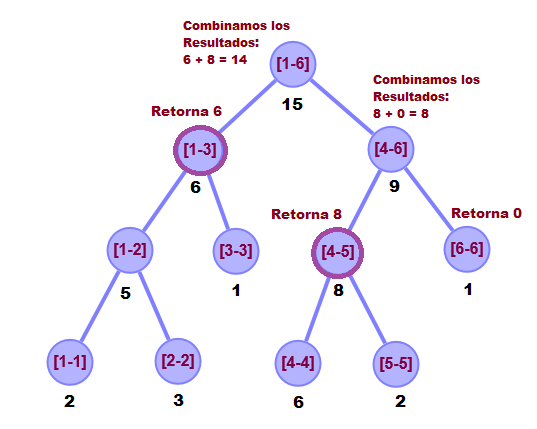
\includegraphics[width=\linewidth]{imag/segment_tree_query_values}
    \label{fig:example_st_casos}
\end{minipage}

\noindent\textit{?`Cu\'al es la complejidad temporal de una consulta en rangos?}\\
En este caso la complejidad temporal depende de la cantidad de nodos que son visitados durante la consulta. Una observaci\'on necesaria, es que en cada nivel del \'arbol visitamos a lo m\'as 4 v\'ertices. Este hecho puede probarse mediante inducci\'on, pero no lo vamos a hacer aqu\'i. 

Si en cada nivel visitamos a lo m\'as  cuatro nodos, y el segment tree tiene a lo m\'as $\log_2(n) + 1$ niveles (porque su altura es a lo m\'as $\log_2(n) + 1$), entonces vamos a visitar en total de $4 \cdot \log_2(n) + 4$ v\'ertices en el peor caso. La complejidad final es $O(\log n)$.